\section{Projective Geometry}

\subsection{Perspectivities of Lines}

\defn{Perspective Transformation}{
    Let \(\ell\) and \(\lambda\) be distinct lines and \(O\) a fixed point on neither. A perspective transformation of the lines, also called a perspectivity or central projection is a map \(p: \ell \to \lambda\) that takes every point \(P \in \ell\) to the point where \(OP\) meets \(\lambda\), if such a point eixsts.
    \begin{center}
        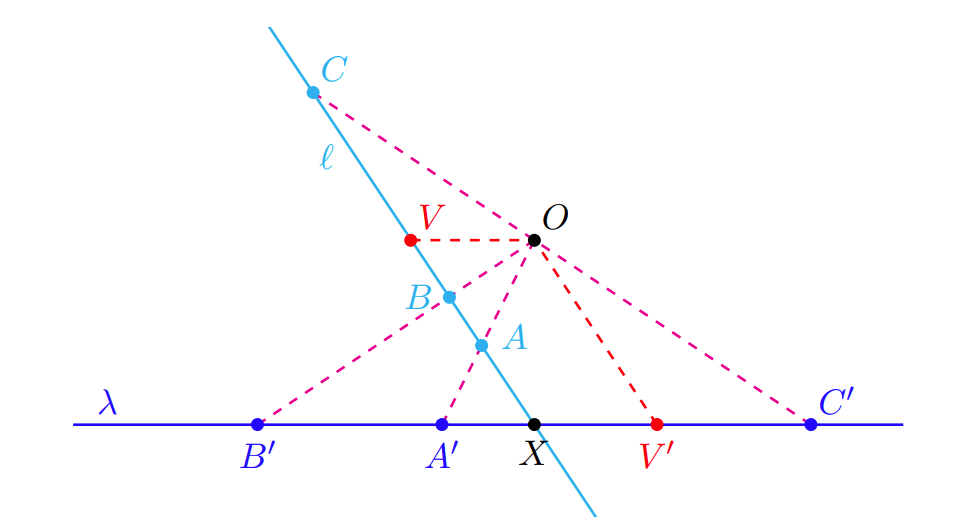
\includegraphics{assets/projective/perspectivity.png}
    \end{center}
}

As the points on \(\ell\) approach \(V\), their images on \(\lambda\) get further and further away to the left until at \(V\), when \(OV\) is parallel to \(\lambda\), the image point vanishes: we call \(V\) the \textbf{vanishing point} on \(\ell\).

\defn{Projectively Extended Real Line}{
    The projectively extended real line, \(\overline{\bR}\) is the set \(\bR \cup \{\infty\}\) where \(\infty\) is the point at infinity.
}

\defn{Projective Transformation}{
    A projective transformation or projectivity is any composition of perspectivities.
}

Any projectivity on a line that has more than two fixed points must be the identity. It also follows that a projectivity of a line to itself is uniquely defined given the images of three distinct points.

\begin{theorem}
    Suppose \(\{A, B, C, D\}\) and \(\{A', B', C', D'\}\) are two sets of four coolinear points (not necessarily in the same plane) such that \([A, B; C, D] = [A', B'; C', D']\). Then there is a projectivity that maps \(A\) to \(A'\) etc.
\end{theorem}

\subsection{Perspectivities of Planes}
\subsection{The Real Projective Plane}
\subsection{Analytic Projective Geometry}